%Searches for CW require a choice of parameters for the global template. For
%narrow band searches we can use EM data to estimate the best choice of
%parameters.  These are found by least-squares fitting a Taylor expansion to the
%observed pulse TOAs, the resulting coefficients are the best fit parameters.
%Peforming a narrow band search for a signal using matched filtering, we
%identify a candidate as a local minimum in mismatch in parameter space. Finding
%such a local minimum can be thought of as a minimisation problem of the
%mismatch with respect to the parameters.  Using the $\mathcal{F}$-statistic
%matched filtering algorithm the phase is analytically minimised by definition.
%Each  parameter that is searched over adds an additional term in the Taylor
%expansion to minimise over.  So searching over $\f$ and $\fdot$ is equivalent
%to analytically minimising with a second order polynomial. To explain this
%better we will use a first look at a generic toy model.

In Sec.~\ref{sec: Defining a random walk} we have defined a random walk model
for which we subsequently calculated the fully-coherent mismatch in
Sec.~\ref{sec: Random walk models part I}. However, this is a special case in
which the random walk for each parameter offsets begins at the origin and then
grows with time. The parameter offsets $\Delta\lambda^{\alpha}$, depend both on
the signal and the template $\lt^{\alpha}$. It is the signal which undergoes a random walk, in Sec.~\ref{sec:
Random walk models part I} we chose the template such that the parameter offset
was zero at the origin. This choice does not minimise the mismatch and therefore
Eqn.~\eqref{eqn: expectation} may overestimate the minimum mismatch
with which the random walk signal could be recovered if we minimised over the
template parameters $\lt^{\alpha}$.

To calculate the minimised mismatch from random walks we first consider
fitting and removing a $k^{th}$-order polynomial from a generic random walk. This
is done in Appendix~\ref{sec: least squares minimisation of a random walk} and
helps to build intuition for the more complicated case of random walk in
GW signals. In the following sections, we will calculate the minimimum
mismatch for random walks in either the phase or frequency (i.e. we do
consider both happening cocurrently, only one at a time).

We will model the parameter offsets $\Delta\phi_{i}, \Delta \f_{i}$
following the definitions in Sec.~\ref{sec: Defining a random walk}.
We will consider a narrow band search in $\f$ and $\fdot$ which is
is equivalent to minimising the mismatch up to a quadratic term in the Taylor
expansion. So the parameter space offsets with which we should calculate the
mismatch from, are given by
\begin{equation}
\Delta^{(2)}\lambda_{\alpha i} = \Delta\lambda_{\alpha i} - \Delta\lambda_{\alpha i}^{2}.
\end{equation}

The generic random walk considered in Appendix~\ref{sec: least squares
minimisation of a random walk} was minimised with respect to the sum of squared
differences between the fit and the random walk. Ideally in calculating the
mismatch we should minimise $\Delta\lambda_{\alpha i}^{2}$ with respect to the
mismatch. However, this adds an additional level of complexity and so we will
consider here the minimisation with respect to the sum of squared differences
which will be similar to the minimisation with respect to the mismatch.

\subsubsection{Random walk in the phase}
We begin with the simplest case of a random walk in phase for which we have
\begin{equation}
\Delta\phi_{i} = \s{j=1}{i}N(0, \sigP).
\end{equation}
Then we note that
\begin{equation}
E[\Delta\phi_{i} \Delta\phi_{j}] = \sigP \min(i, j).
\end{equation}
The mismatch for a random walk in the phase having removed a second order
fit is given by
\begin{align}
\mutilde & = g_{\alpha \beta i j} \Delta^{(2)}\lambda^{\alpha i}\Delta^{(2)}\lambda^{\beta j} \\
& = \s{i=1}{N}g_{00}^{E} \Delta^{(2)}\phi_{i}\Delta^{(2)}\phi_{i}
+ 2 \s{i=1}{N}\s{j=1}{i-1}g_{00}^{NE}\Delta^{(2)}\phi_{i}\Delta^{(2)}\phi_{j}.
\label{eqn: 4202540871}
\end{align}
To calculate the expectation of the mismatch, we need to evaluate the
expectation of
\begin{align}
\Delta^{(2)}\phi_{i}\Delta^{(2)}\phi_{i} = & \left(\Delta\phi_{i}
- \s{k=1}{N}\CT_{ik}\Delta\phi_{k}\right)
 \left(\Delta\phi_{j} - \s{l=1}{N}\CT_{jl}\Delta\phi_{l}\right) \\
\begin{split}
= & \Delta\phi_{i}\Delta\phi_{j} -
\left(\s{k=1}{N}\CT_{ik} \Delta\phi_{j}\Delta\phi_{k}
+ \s{l=1}{N}\CT_{jl}\Delta\phi_{i}\Delta\phi_{l}\right) \\
& +
\s{k=1}{N}\s{l=1}{N}\CT_{ik}\CT_{jl} \Delta\phi_{k}\Delta\phi_{l},
\end{split}
\end{align}
where $\CT_{ij}$ is defined Eqn.~\ref{eqn: C_2} and Eqn.~\ref{eqn:  MCC_2}
and we have replaced $\Delta x$ with the time $\dT$. Then taking the expectation
\begin{align}
\E{\Delta^{(2)}\phi_{i}\Delta^{(2)}\phi_{i}} & =
%E\left[\Delta\phi_{i}\Delta\phi_{j}\right] -
%\left(\s{k=1}{N}E[\Delta\phi_{j}\Delta\phi_{k}]
%+ \s{l=1}{N}E[\Delta\phi_{i}\Delta\phi_{l}]\right) +
%\s{k=1}{N}\s{l=1}{N}E[\Delta\phi_{k}\Delta\phi_{l}]\\
%& = 
\sigma^{2}_{\phi} \left(\min(i, j) - \left(\s{k=1}{N}\CT_{ik} \min(j, k)
+ \s{l=1}{N}\CT_{jl}\min(i, l) \right)\right. \notag \\
& \hspace{13mm} \left. + \s{k=1}{N}\s{l=1}{N}\CT_{ik}\CT_{jl}\min(k, l)\right).
\label{eqn: expected mismatch dP0idP0j_k2}
\end{align}
Using symbolic mathematics packages we
calculate an analytic expression which is a function of $\dT, i, j$ and $N$.
Inserting this into Eqn.~\eqref{eqn: 4202540871} and simplifying we find that
\begin{align}
E[\mutilde]  & = \s{i=1}{N}g_{00}^{E} E\left[\Delta^{(2)}\phi_{i}\Delta^{(2)}\phi_{i}\right]
+ 2 \s{i=1}{N}\s{j=1}{i-1}g_{00}^{NE}E\left[\Delta^{(2)}\phi_{i}\Delta^{(2)}\phi_{j}\right]  \\
& = \frac{1}{70}\sigP\left(3N - \frac{27}{N}\right).
\label{eqn: Expected mismatch RW in phase k2}
\end{align}
This expression can be compared to Eqn.~\eqref{eqn: expectation} ignoring the
effect of the random walk in spin-down rate. Notably, we retain the same
leading order scaling of $N$, but the overall coefficient is decreased.
Rearranging the expression in the bracket demonstrates the mismatch is negative
or zero for $1 \ge N \ge 3$: this is a reflection of the minimum number of
points needed in order to perform the quadratic fit.

\subsubsection{Random walk in the frequency}

For a random walk in the frequency we have an added complexity caused by the
effect the frequency offsets induces in the phase. For the frequency offset we
have
\begin{align}
\Delta f_{i} &= \s{j=1}{i}N(0, \sigF).
\end{align}
Recalling that we set the reference time at the beginning of each segment,
then as in Sec.~\ref{sec: Defining a random walk}, the induced phase offset is
\begin{align}
\Delta\phi_{i} &=2\pi \s{j=1}{i-1}f_{j}\dT \\
 & = 2\pi\dT \s{j=1}{i-1}\s{k=1}{j}N(0, \sigF) \\
& = 2\pi\dT \s{j=1}{i}(i-j)N(0, \sigF).
\end{align}
The expected values of combinations of these quantities we find to be
\begin{align}
E[\Delta\f_{i}\Delta\f_{j}] & = \sigF \min(i, j), \\
E[\Delta\phi_{i}\Delta\f_{j}] & = 2 \pi \dT \sigF \s{k=1}{\min(i, j)}(i-k),\\
E[\Delta\phi_{i}\Delta\phi_{j}] & =
\left(2\pi\dT\right)^{2}\sigF \s{k=1}{\min(i, j)}(i-k)(j-k).
\label{eqn: Expectations raw}
\end{align}
Then calculating the expected mismatch due to a random walk in frequency
\begin{align}
\begin{split}
E[\mutilde] = &
\s{i=1}{N}\left(g_{00}^{E}E\left[\Delta^{(2)}\phi_{i}\Delta^{(2)}\phi_{i}\right]
+ 2 g_{01}^{E}E\left[\Delta^{(2)}\phi_{i}\Delta^{(2)}\f_{i}\right]
+  g_{11}^{E} E\left[\Delta^{(2)}\f_{i}\Delta^{(2)}\f_{i}\right] \right) \\
& + 2\s{i=1}{N}\s{j=1}{i-1}\left(\right.
g_{00}^{NE}E\left[\Delta^{(2)}\phi_{i}\Delta^{(2)}\phi_{j}\right] +
g_{01}^{NE}E\left[\Delta^{(2)}\phi_{j}\Delta^{(2)}\f_{i}\right] +  \\
&\hspace{20mm}\left. g_{10}^{NE}E\left[\Delta^{(2)}\phi_{i}\Delta^{(2)}\f_{j}\right] +
g_{11}^{NE} E\left[\Delta^{(2)}\f_{i}\Delta^{(2)}\f_{j}\right] \right).
\end{split}
\end{align}
We calculate each of these expressions in a similar manner to Eqn.~\eqref{eqn:
expected mismatch dP0idP0j_k2} replacing the relevant expectations with those
given in Eqn.~\eqref{eqn: Expectations raw}. This yields an expected
mismatch given by
\begin{equation}
E[\mutilde] = \frac{\pi^{2} }{630} \sigF \dT^{2}  \left(N^{3} - 7N- \frac{18}{N} \right).
\label{eqn: Expected mismatch RW in frequency k2}
\end{equation}
Again this can be compared with Eqn.~\eqref{eqn: expectation} ignorring the
mismatch due to the random walk in the spin-down rate.

\subsubsection{Verification}

We now verify Eqn.~\eqref{eqn: Expected mismatch RW in frequency k2} and
Eqn.~\eqref{eqn: Expected mismatch RW in phase k2} by comparing with Monte
Carlo simulations. The numerical signals undergo a random walk as described in
Sec.~\ref{sec: Random walk models part I}, however, when searching for the
signals we search over a grid of points in $f$ and $\dot{f}$ then select grid point
with the minimum mismatch; this effectively minimises over the frequency and
spin-down. The results are plotted in Fig.~\ref{fig: verification of
minimised RW} and demonstrate good agreement between the analytic and simulated
mismatches.

\begin{figure}[ht]
\centering
\subfloat[Random walk in phase]{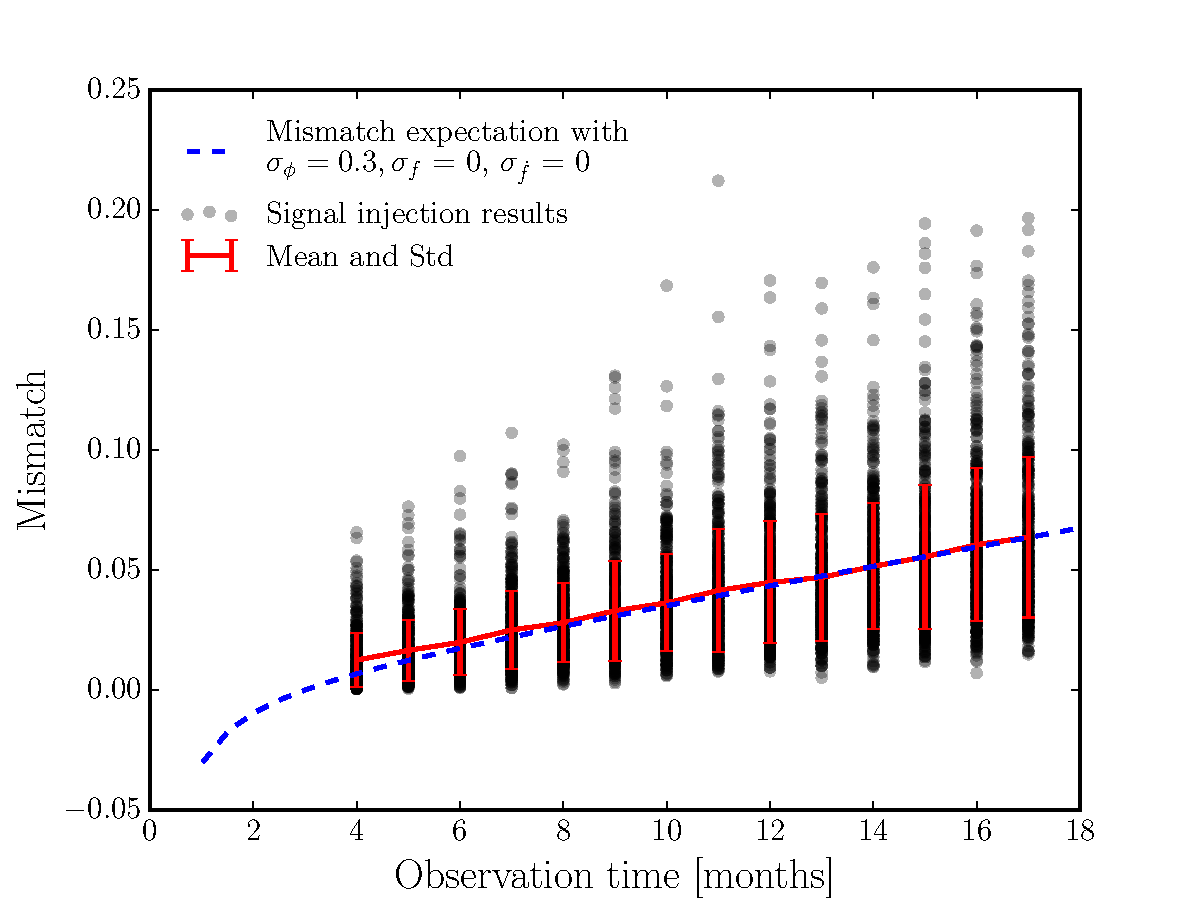
\includegraphics[width=0.5\textwidth]{ExpectationPhase_NarrowBand}}
\subfloat[Random walk in frequency]{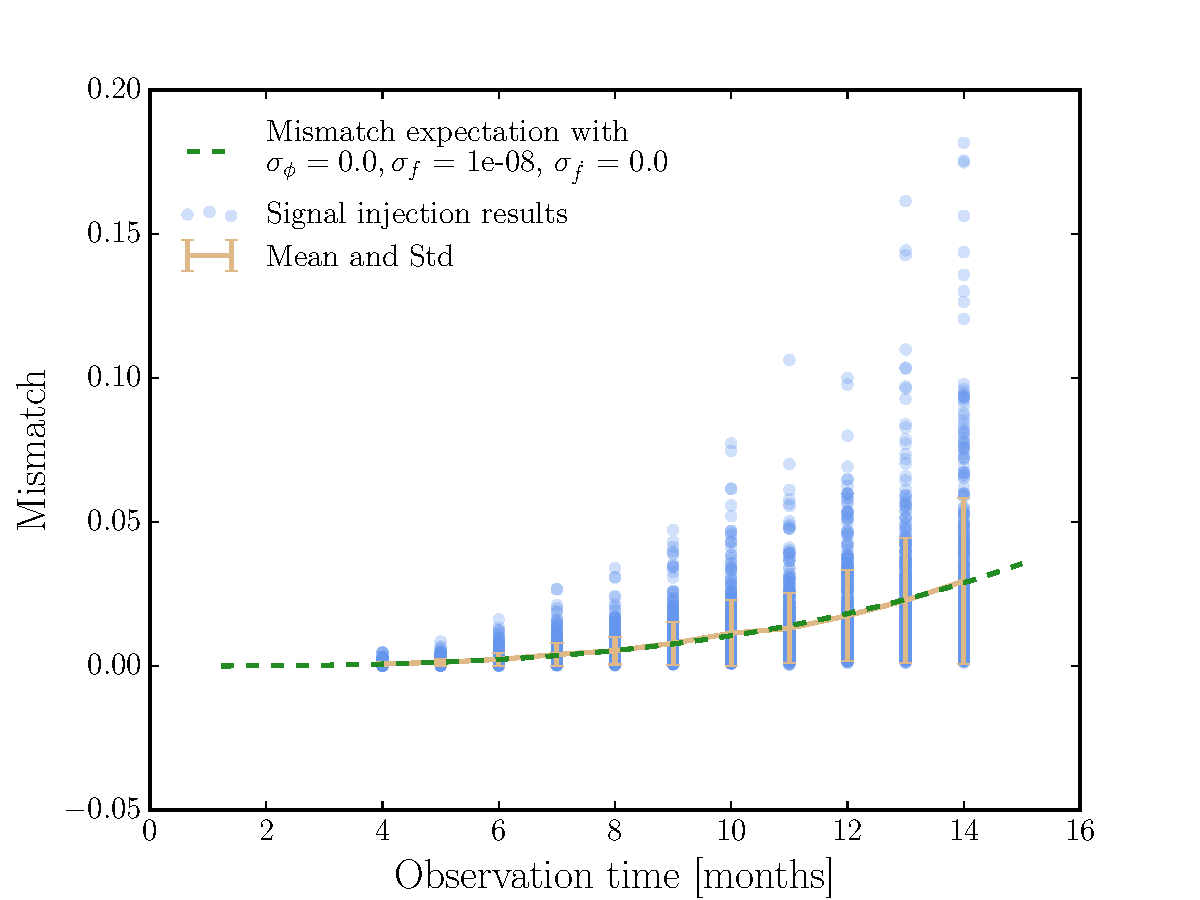
\includegraphics[width=0.5\textwidth]{ExpectationFrequency_NarrowBand}}\\
%\subfloat[Random walk in spin-down]{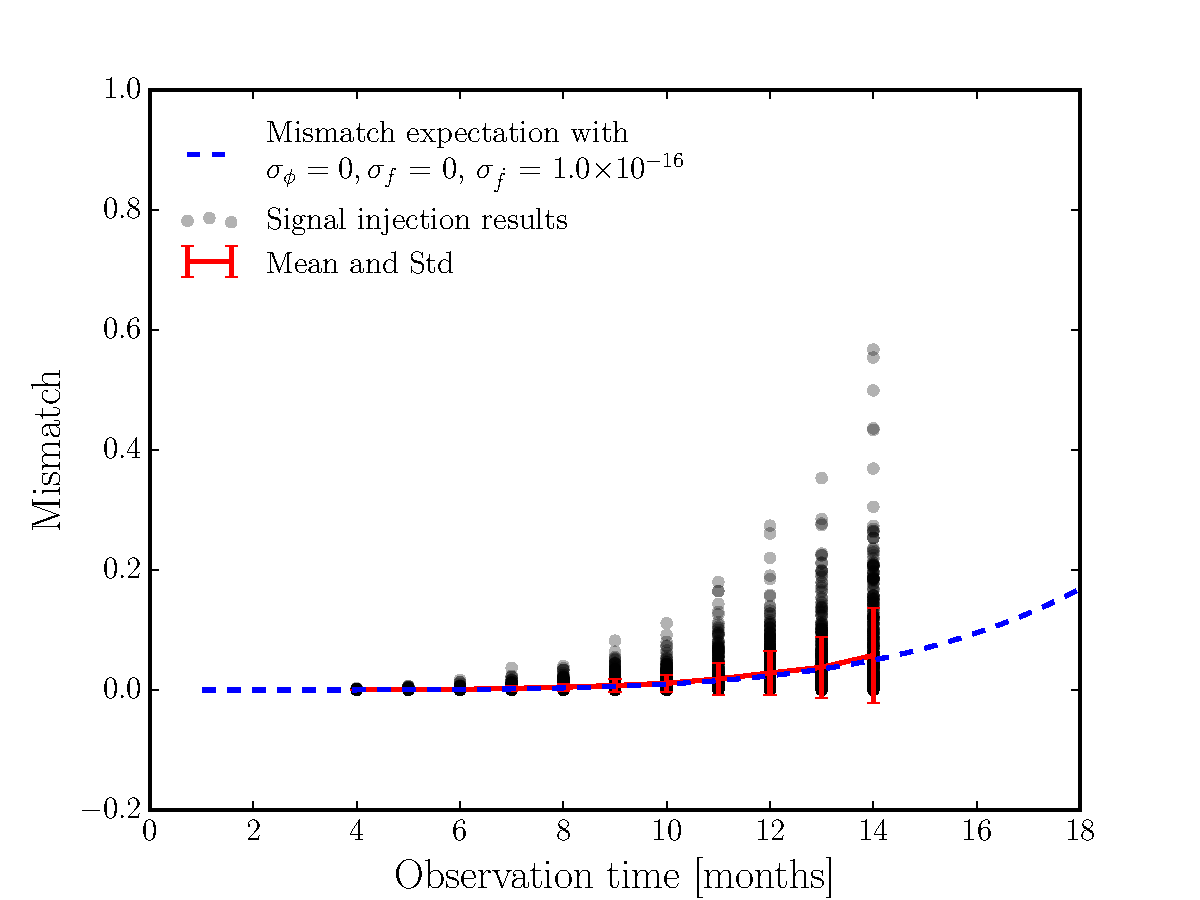
\includegraphics[width=0.5\textwidth]{ExpectationSpindown}}
\caption{A comparison of the Monto Carlo numerical simulated mismatch with the
predictions of Eqn.~\eqref{eqn: Expected mismatch RW in
frequency k2} and Eqn.~\eqref{eqn: Expected mismatch RW in phase k2}; this differs
from Fig.~\ref{fig: rw I} in that the numerical mismatch is minimised by selecting
the smallest mismatch from a grid of points in $f$ and $\dot{f}$.}
\label{fig: verification of minimised RW}
\end{figure}•
\FloatBarrier
